\textcolor{teal}{\textbf{real-life scenario.}} We illustrate our framework for autonomous vehicle path planning in environments with uncertain elements. An uncertain object's diameter and probability is modeled as a subgraph with weighted edges. Navigating through uncertain conditions, minimizing total probabilistic expectation, is accounted by finding a shortest-weight path. See \textit{Figure 1} for a vehicle's environment's object detection.

\textcolor{teal}{\textbf{math notation within a real-life context.}}

\textcolor{teal}{\textbf{graph.}} A vehicle's possible paths may be thought of by a set of discrete waypoints, whereby each waypoint allows the transition to some other waypoints. In terms of graph theory, it is a digraph $G$ where waypoints correspond to vertices $V(G)$, and valid transitions are given by directed edges $E(G)$. An edge $(a,b)$ indicates a transition from waypoint $a$ to waypoint $b$ is possible.

\textcolor{teal}{\textbf{classification.}} An object's uncertain classification is given by a probability distribution over classes. For example we may classify an object as either a dog with probability 0.7 or a cat with probability 0.3. Likelihoods and penalties could be combined by probabilistic expectation $Ex[X]$. For example, the expected harm or penalty is $Ex[X] = (2 \cdot 0.3) + (1 \cdot 0.7)$ given cats are twice as important or penalizing as dogs. A vertex weight $w(v)$ is set with such expectation denoting classification uncertainty.

\textcolor{teal}{\textbf{positioning.}} An object's uncertain position corresponds to potential subset of vertices, which we call an uncertain subgraph $U$. Since the object is known to exist, vertices of $U$ constitute a probability distribution. For example, if an object's position may be uniformly uncertain among nearby vertices $v_1, v_2, v_3, v_4, v_5$ where $(v_1,v_2), (v_1, v_3), (v_1, v_4), (v_5,v_1) \in E(G)$. Similarly, a constant penalty, since it is the same object, may be set for all vertices of $U$.

\textcolor{teal}{\textbf{path.}} We will prove later it is equivalent to set a weight for edge $(a,b)$ in place of vertex $b$ weight. By linearity of expectation, the total probabilistic expectation of a path is the summation of edges' weights the path navigates through. It follows, computing a shortest path suffices for minimizing the total expectation.

\begin{center}
  \includegraphics[width=0.75\textwidth]{images/sensor.png} \\
  Figure 1:  Vehicle's detected environment \footnote{taken from \cite{sensor}}.
\end{center}

\textcolor{teal}{\textbf{precise formal definition}}

We are given a simple directed graph $G$. That is, a set $V$ together with an irreflexive binary relation $E$ on $V$. We call them vertices and directed edges. Our digraphs are anti-symmetric between any two vertices. The sample space $\Omega$ is the set of all possible objects at some waypoint. By convention, no two objects are present in the same waypoint, so $Pr[E] = 0$ for all $E \subseteq \Omega$ where $|E| \geq 2$. A random variable $X$ associates a penalty for each outcome, and the corresponding random variable distribution $\mu_X$ associates probabilities for outcomes.

\textbf{Definition.} For a subset of vertices $S = \{ v_1, \dots, v_k \} \subseteq V(G)$ and a set of random variable distributions $\{ \mu_{X_1}, \dots, \mu_{X_k} \}$, an \textit{uncertain zone} is a function $U$
$$
U: v_i \mapsto \mu_{X_i}.
$$

\textbf{Examples.} See \textit{Figure 2} for a visualizing aid.
\begin{itemize}
    \item \textit{Case 1.} $U = \{ (v_8, \{(1, 0.7)\} ) \}$ denotes an object is present in some vertex $v_8$ with probability $0.7$.
    \item \textit{Case 2.} $U = \{ (v_8, \{(1, 0.3)\}), (v_{12}, \{(1, 0.3)\}), (v_{14}, \{(1, 0.3)\}) \}$ denotes an object is present in one of vertices $v_8$, $v_{12}$, and $v_{14}$, each with probability $0.3$.
    \item \textit{Case 3.} $U = \{ (v_8, \{ (100, 0.5), (5, 0.5) \} ) \}$ denotes $v_8$ either has a box with probability $0.5$ and penalty $5$, or a pedestrian with probability $0.5$ and penalty $100$.
\end{itemize}

\textbf{Definition.} "given an uncertain zone" "number definitions". Since each $X$ induces $Ex[X]$ on a vertex, an \textit{uncertain environment} is declared to be a tuple $(G, h:V(G) \rightarrow \mathbb{R} )$, of a digraph $G$ and a partial function $h$ labeling vertices.

\tikzset{every picture/.style={line width=0.75pt}} %set default line width to 0.75pt        

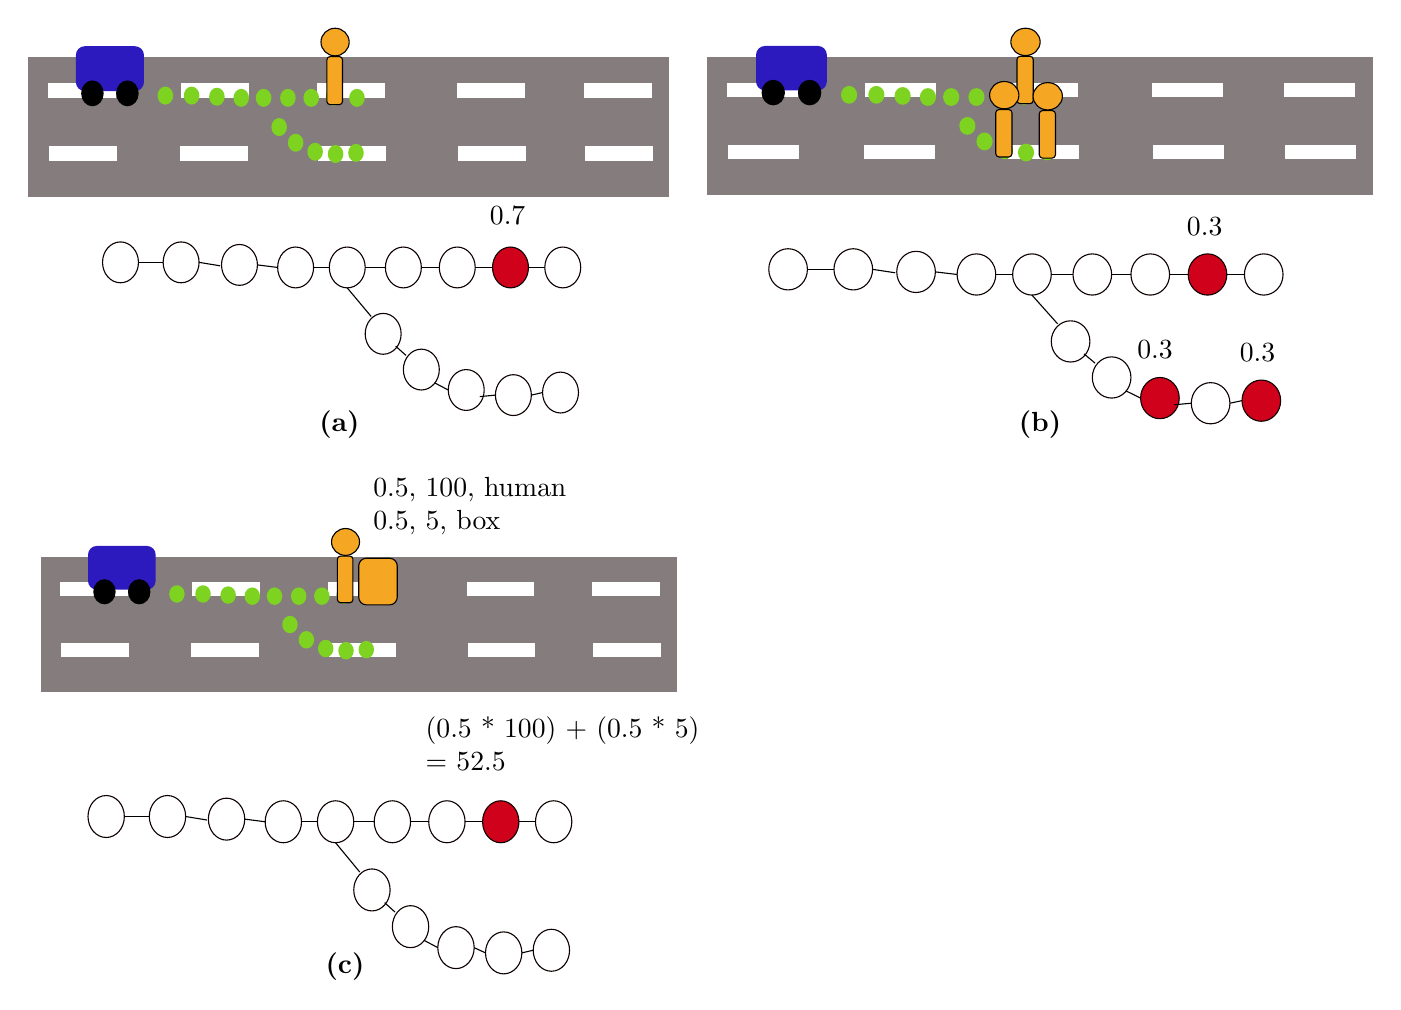
\begin{tikzpicture}[x=0.75pt,y=0.75pt,yscale=-1,xscale=1]
%uncomment if require: \path (0,483); %set diagram left start at 0, and has height of 483

%Shape: Rectangle [id:dp7528609936411457] 
\draw  [draw opacity=0][fill={rgb, 255:red, 133; green, 125; blue, 125 }  ,fill opacity=1 ] (7,24.07) -- (315.8,24.07) -- (315.8,57.61) -- (7,57.61) -- cycle ;
%Shape: Rectangle [id:dp8661548351503254] 
\draw  [draw opacity=0][fill={rgb, 255:red, 255; green, 255; blue, 255 }  ,fill opacity=1 ] (16.37,36.51) -- (49.17,36.51) -- (49.17,43.54) -- (16.37,43.54) -- cycle ;
%Shape: Rectangle [id:dp10859990436091471] 
\draw  [draw opacity=0][fill={rgb, 255:red, 255; green, 255; blue, 255 }  ,fill opacity=1 ] (80.57,36.51) -- (113.37,36.51) -- (113.37,43.54) -- (80.57,43.54) -- cycle ;
%Shape: Rectangle [id:dp268899859234089] 
\draw  [draw opacity=0][fill={rgb, 255:red, 255; green, 255; blue, 255 }  ,fill opacity=1 ] (146.17,36.51) -- (178.97,36.51) -- (178.97,43.54) -- (146.17,43.54) -- cycle ;
%Shape: Rectangle [id:dp899055447989638] 
\draw  [draw opacity=0][fill={rgb, 255:red, 255; green, 255; blue, 255 }  ,fill opacity=1 ] (213.65,36.51) -- (246.45,36.51) -- (246.45,43.54) -- (213.65,43.54) -- cycle ;
%Shape: Rectangle [id:dp480508071363392] 
\draw  [draw opacity=0][fill={rgb, 255:red, 255; green, 255; blue, 255 }  ,fill opacity=1 ] (274.56,36.51) -- (307.37,36.51) -- (307.37,43.54) -- (274.56,43.54) -- cycle ;
%Rounded Rect [id:dp32018534560807566] 
\draw  [draw opacity=0][fill={rgb, 255:red, 44; green, 26; blue, 190 }  ,fill opacity=1 ] (29.96,22.98) .. controls (29.96,20.59) and (31.9,18.66) .. (34.29,18.66) -- (58.43,18.66) .. controls (60.82,18.66) and (62.76,20.59) .. (62.76,22.98) -- (62.76,35.97) .. controls (62.76,38.36) and (60.82,40.3) .. (58.43,40.3) -- (34.29,40.3) .. controls (31.9,40.3) and (29.96,38.36) .. (29.96,35.97) -- cycle ;
%Shape: Ellipse [id:dp18078733203462516] 
\draw  [fill={rgb, 255:red, 0; green, 0; blue, 0 }  ,fill opacity=1 ] (32.77,41.38) .. controls (32.77,38.09) and (35.08,35.43) .. (37.93,35.43) .. controls (40.77,35.43) and (43.08,38.09) .. (43.08,41.38) .. controls (43.08,44.67) and (40.77,47.33) .. (37.93,47.33) .. controls (35.08,47.33) and (32.77,44.67) .. (32.77,41.38) -- cycle ;
%Shape: Ellipse [id:dp21140757651539777] 
\draw  [fill={rgb, 255:red, 0; green, 0; blue, 0 }  ,fill opacity=1 ] (49.64,41.38) .. controls (49.64,38.09) and (51.95,35.43) .. (54.8,35.43) .. controls (57.64,35.43) and (59.95,38.09) .. (59.95,41.38) .. controls (59.95,44.67) and (57.64,47.33) .. (54.8,47.33) .. controls (51.95,47.33) and (49.64,44.67) .. (49.64,41.38) -- cycle ;

%Shape: Ellipse [id:dp778751357944039] 
\draw  [draw opacity=0][fill={rgb, 255:red, 126; green, 211; blue, 33 }  ,fill opacity=1 ] (69.32,42.46) .. controls (69.32,40.07) and (71,38.13) .. (73.07,38.13) .. controls (75.14,38.13) and (76.82,40.07) .. (76.82,42.46) .. controls (76.82,44.85) and (75.14,46.79) .. (73.07,46.79) .. controls (71,46.79) and (69.32,44.85) .. (69.32,42.46) -- cycle ;
%Shape: Ellipse [id:dp06448410533004156] 
\draw  [draw opacity=0][fill={rgb, 255:red, 126; green, 211; blue, 33 }  ,fill opacity=1 ] (81.97,42.46) .. controls (81.97,40.07) and (83.65,38.13) .. (85.72,38.13) .. controls (87.79,38.13) and (89.47,40.07) .. (89.47,42.46) .. controls (89.47,44.85) and (87.79,46.79) .. (85.72,46.79) .. controls (83.65,46.79) and (81.97,44.85) .. (81.97,42.46) -- cycle ;
%Shape: Ellipse [id:dp02600584247194737] 
\draw  [draw opacity=0][fill={rgb, 255:red, 126; green, 211; blue, 33 }  ,fill opacity=1 ] (94.16,43) .. controls (94.16,40.61) and (95.84,38.67) .. (97.91,38.67) .. controls (99.98,38.67) and (101.65,40.61) .. (101.65,43) .. controls (101.65,45.39) and (99.98,47.33) .. (97.91,47.33) .. controls (95.84,47.33) and (94.16,45.39) .. (94.16,43) -- cycle ;
%Shape: Ellipse [id:dp18305244714220947] 
\draw  [draw opacity=0][fill={rgb, 255:red, 126; green, 211; blue, 33 }  ,fill opacity=1 ] (105.87,43.54) .. controls (105.87,41.15) and (107.55,39.22) .. (109.62,39.22) .. controls (111.69,39.22) and (113.37,41.15) .. (113.37,43.54) .. controls (113.37,45.93) and (111.69,47.87) .. (109.62,47.87) .. controls (107.55,47.87) and (105.87,45.93) .. (105.87,43.54) -- cycle ;
%Shape: Ellipse [id:dp4876586592944341] 
\draw  [draw opacity=0][fill={rgb, 255:red, 126; green, 211; blue, 33 }  ,fill opacity=1 ] (116.65,43.54) .. controls (116.65,41.15) and (118.33,39.22) .. (120.4,39.22) .. controls (122.47,39.22) and (124.15,41.15) .. (124.15,43.54) .. controls (124.15,45.93) and (122.47,47.87) .. (120.4,47.87) .. controls (118.33,47.87) and (116.65,45.93) .. (116.65,43.54) -- cycle ;
%Shape: Ellipse [id:dp9543782055147612] 
\draw  [draw opacity=0][fill={rgb, 255:red, 126; green, 211; blue, 33 }  ,fill opacity=1 ] (128.36,43.54) .. controls (128.36,41.15) and (130.04,39.22) .. (132.11,39.22) .. controls (134.18,39.22) and (135.86,41.15) .. (135.86,43.54) .. controls (135.86,45.93) and (134.18,47.87) .. (132.11,47.87) .. controls (130.04,47.87) and (128.36,45.93) .. (128.36,43.54) -- cycle ;
%Shape: Ellipse [id:dp9791446263778842] 
\draw  [draw opacity=0][fill={rgb, 255:red, 126; green, 211; blue, 33 }  ,fill opacity=1 ] (139.61,43.54) .. controls (139.61,41.15) and (141.29,39.22) .. (143.36,39.22) .. controls (145.43,39.22) and (147.11,41.15) .. (147.11,43.54) .. controls (147.11,45.93) and (145.43,47.87) .. (143.36,47.87) .. controls (141.29,47.87) and (139.61,45.93) .. (139.61,43.54) -- cycle ;
%Shape: Ellipse [id:dp4568300815477506] 
\draw  [draw opacity=0][fill={rgb, 255:red, 126; green, 211; blue, 33 }  ,fill opacity=1 ] (150.39,43) .. controls (150.39,40.61) and (152.07,38.67) .. (154.14,38.67) .. controls (156.21,38.67) and (157.89,40.61) .. (157.89,43) .. controls (157.89,45.39) and (156.21,47.33) .. (154.14,47.33) .. controls (152.07,47.33) and (150.39,45.39) .. (150.39,43) -- cycle ;
%Shape: Ellipse [id:dp709493426596874] 
\draw  [draw opacity=0][fill={rgb, 255:red, 126; green, 211; blue, 33 }  ,fill opacity=1 ] (161.63,43.54) .. controls (161.63,41.15) and (163.31,39.22) .. (165.38,39.22) .. controls (167.45,39.22) and (169.13,41.15) .. (169.13,43.54) .. controls (169.13,45.93) and (167.45,47.87) .. (165.38,47.87) .. controls (163.31,47.87) and (161.63,45.93) .. (161.63,43.54) -- cycle ;
%Shape: Rectangle [id:dp3078801108110205] 
\draw  [draw opacity=0][fill={rgb, 255:red, 133; green, 125; blue, 125 }  ,fill opacity=1 ] (7,57.61) -- (315.8,57.61) -- (315.8,91.15) -- (7,91.15) -- cycle ;
%Shape: Rectangle [id:dp39691407928367517] 
\draw  [draw opacity=0][fill={rgb, 255:red, 255; green, 255; blue, 255 }  ,fill opacity=1 ] (146.64,66.81) -- (179.44,66.81) -- (179.44,73.84) -- (146.64,73.84) -- cycle ;
%Shape: Rectangle [id:dp6342125577335092] 
\draw  [draw opacity=0][fill={rgb, 255:red, 255; green, 255; blue, 255 }  ,fill opacity=1 ] (214.12,66.81) -- (246.92,66.81) -- (246.92,73.84) -- (214.12,73.84) -- cycle ;
%Shape: Rectangle [id:dp03384397152413832] 
\draw  [draw opacity=0][fill={rgb, 255:red, 255; green, 255; blue, 255 }  ,fill opacity=1 ] (275.03,66.81) -- (307.83,66.81) -- (307.83,73.84) -- (275.03,73.84) -- cycle ;
%Shape: Rectangle [id:dp1856018926226921] 
\draw  [draw opacity=0][fill={rgb, 255:red, 255; green, 255; blue, 255 }  ,fill opacity=1 ] (16.84,66.81) -- (49.64,66.81) -- (49.64,73.84) -- (16.84,73.84) -- cycle ;
%Shape: Rectangle [id:dp05371870608898166] 
\draw  [draw opacity=0][fill={rgb, 255:red, 255; green, 255; blue, 255 }  ,fill opacity=1 ] (80.1,66.81) -- (112.9,66.81) -- (112.9,73.84) -- (80.1,73.84) -- cycle ;
%Shape: Ellipse [id:dp31499498471483345] 
\draw  [draw opacity=0][fill={rgb, 255:red, 126; green, 211; blue, 33 }  ,fill opacity=1 ] (124.15,57.61) .. controls (124.15,55.22) and (125.83,53.28) .. (127.9,53.28) .. controls (129.97,53.28) and (131.64,55.22) .. (131.64,57.61) .. controls (131.64,60) and (129.97,61.94) .. (127.9,61.94) .. controls (125.83,61.94) and (124.15,60) .. (124.15,57.61) -- cycle ;
%Shape: Ellipse [id:dp18385916317182405] 
\draw  [draw opacity=0][fill={rgb, 255:red, 126; green, 211; blue, 33 }  ,fill opacity=1 ] (132.11,65.18) .. controls (132.11,62.79) and (133.79,60.86) .. (135.86,60.86) .. controls (137.93,60.86) and (139.61,62.79) .. (139.61,65.18) .. controls (139.61,67.57) and (137.93,69.51) .. (135.86,69.51) .. controls (133.79,69.51) and (132.11,67.57) .. (132.11,65.18) -- cycle ;
%Shape: Ellipse [id:dp6141701799508046] 
\draw  [draw opacity=0][fill={rgb, 255:red, 126; green, 211; blue, 33 }  ,fill opacity=1 ] (141.48,69.51) .. controls (141.48,67.12) and (143.16,65.18) .. (145.23,65.18) .. controls (147.3,65.18) and (148.98,67.12) .. (148.98,69.51) .. controls (148.98,71.9) and (147.3,73.84) .. (145.23,73.84) .. controls (143.16,73.84) and (141.48,71.9) .. (141.48,69.51) -- cycle ;
%Shape: Ellipse [id:dp7059117586429557] 
\draw  [draw opacity=0][fill={rgb, 255:red, 126; green, 211; blue, 33 }  ,fill opacity=1 ] (151.33,70.59) .. controls (151.33,68.2) and (153,66.27) .. (155.07,66.27) .. controls (157.14,66.27) and (158.82,68.2) .. (158.82,70.59) .. controls (158.82,72.98) and (157.14,74.92) .. (155.07,74.92) .. controls (153,74.92) and (151.33,72.98) .. (151.33,70.59) -- cycle ;
%Shape: Ellipse [id:dp9498127525041196] 
\draw  [draw opacity=0][fill={rgb, 255:red, 126; green, 211; blue, 33 }  ,fill opacity=1 ] (161.17,70.05) .. controls (161.17,67.66) and (162.84,65.73) .. (164.91,65.73) .. controls (166.98,65.73) and (168.66,67.66) .. (168.66,70.05) .. controls (168.66,72.44) and (166.98,74.38) .. (164.91,74.38) .. controls (162.84,74.38) and (161.17,72.44) .. (161.17,70.05) -- cycle ;
%Shape: Ellipse [id:dp5154539478659079] 
\draw  [color={rgb, 255:red, 0; green, 0; blue, 0 }  ,draw opacity=1 ][fill={rgb, 255:red, 245; green, 166; blue, 35 }  ,fill opacity=1 ] (148.05,16.66) .. controls (148.05,12.98) and (151.09,10) .. (154.84,10) .. controls (158.59,10) and (161.63,12.98) .. (161.63,16.66) .. controls (161.63,20.33) and (158.59,23.31) .. (154.84,23.31) .. controls (151.09,23.31) and (148.05,20.33) .. (148.05,16.66) -- cycle ;
%Rounded Rect [id:dp4882504435042905] 
\draw  [color={rgb, 255:red, 0; green, 0; blue, 0 }  ,draw opacity=1 ][fill={rgb, 255:red, 245; green, 166; blue, 35 }  ,fill opacity=1 ] (150.91,25.17) .. controls (150.91,24.34) and (151.58,23.66) .. (152.41,23.66) -- (156.91,23.66) .. controls (157.74,23.66) and (158.42,24.34) .. (158.42,25.17) -- (158.42,45.29) .. controls (158.42,46.12) and (157.74,46.79) .. (156.91,46.79) -- (152.41,46.79) .. controls (151.58,46.79) and (150.91,46.12) .. (150.91,45.29) -- cycle ;

%Shape: Ellipse [id:dp9103409908276086] 
\draw  [color={rgb, 255:red, 14; green, 0; blue, 0 }  ,draw opacity=1 ] (42.8,122.8) .. controls (42.8,117.37) and (46.67,112.96) .. (51.45,112.96) .. controls (56.23,112.96) and (60.11,117.37) .. (60.11,122.8) .. controls (60.11,128.24) and (56.23,132.64) .. (51.45,132.64) .. controls (46.67,132.64) and (42.8,128.24) .. (42.8,122.8) -- cycle ;
%Shape: Ellipse [id:dp740083289005012] 
\draw  [color={rgb, 255:red, 14; green, 0; blue, 0 }  ,draw opacity=1 ] (72,122.8) .. controls (72,117.37) and (75.88,112.96) .. (80.66,112.96) .. controls (85.44,112.96) and (89.31,117.37) .. (89.31,122.8) .. controls (89.31,128.24) and (85.44,132.64) .. (80.66,132.64) .. controls (75.88,132.64) and (72,128.24) .. (72,122.8) -- cycle ;
%Shape: Ellipse [id:dp9541917593446743] 
\draw  [color={rgb, 255:red, 14; green, 0; blue, 0 }  ,draw opacity=1 ] (100.13,124.03) .. controls (100.13,118.6) and (104,114.19) .. (108.78,114.19) .. controls (113.56,114.19) and (117.43,118.6) .. (117.43,124.03) .. controls (117.43,129.47) and (113.56,133.87) .. (108.78,133.87) .. controls (104,133.87) and (100.13,129.47) .. (100.13,124.03) -- cycle ;
%Shape: Ellipse [id:dp1856273890999922] 
\draw  [color={rgb, 255:red, 14; green, 0; blue, 0 }  ,draw opacity=1 ] (127.17,125.26) .. controls (127.17,119.83) and (131.04,115.42) .. (135.82,115.42) .. controls (140.6,115.42) and (144.48,119.83) .. (144.48,125.26) .. controls (144.48,130.7) and (140.6,135.1) .. (135.82,135.1) .. controls (131.04,135.1) and (127.17,130.7) .. (127.17,125.26) -- cycle ;
%Shape: Ellipse [id:dp9526061796743859] 
\draw  [color={rgb, 255:red, 14; green, 0; blue, 0 }  ,draw opacity=1 ] (152.05,125.26) .. controls (152.05,119.83) and (155.92,115.42) .. (160.7,115.42) .. controls (165.48,115.42) and (169.35,119.83) .. (169.35,125.26) .. controls (169.35,130.7) and (165.48,135.1) .. (160.7,135.1) .. controls (155.92,135.1) and (152.05,130.7) .. (152.05,125.26) -- cycle ;
%Shape: Ellipse [id:dp06700862762782633] 
\draw  [color={rgb, 255:red, 14; green, 0; blue, 0 }  ,draw opacity=1 ] (179.09,125.26) .. controls (179.09,119.83) and (182.96,115.42) .. (187.74,115.42) .. controls (192.52,115.42) and (196.4,119.83) .. (196.4,125.26) .. controls (196.4,130.7) and (192.52,135.1) .. (187.74,135.1) .. controls (182.96,135.1) and (179.09,130.7) .. (179.09,125.26) -- cycle ;
%Shape: Ellipse [id:dp044156064147011787] 
\draw  [color={rgb, 255:red, 14; green, 0; blue, 0 }  ,draw opacity=1 ] (205.05,125.26) .. controls (205.05,119.83) and (208.92,115.42) .. (213.7,115.42) .. controls (218.48,115.42) and (222.36,119.83) .. (222.36,125.26) .. controls (222.36,130.7) and (218.48,135.1) .. (213.7,135.1) .. controls (208.92,135.1) and (205.05,130.7) .. (205.05,125.26) -- cycle ;
%Shape: Ellipse [id:dp3314667114495382] 
\draw  [color={rgb, 255:red, 14; green, 0; blue, 0 }  ,draw opacity=1 ] (255.89,125.26) .. controls (255.89,119.83) and (259.76,115.42) .. (264.54,115.42) .. controls (269.32,115.42) and (273.19,119.83) .. (273.19,125.26) .. controls (273.19,130.7) and (269.32,135.1) .. (264.54,135.1) .. controls (259.76,135.1) and (255.89,130.7) .. (255.89,125.26) -- cycle ;
%Shape: Ellipse [id:dp6843056607618183] 
\draw  [color={rgb, 255:red, 14; green, 0; blue, 0 }  ,draw opacity=1 ] (169.35,157.24) .. controls (169.35,151.81) and (173.23,147.4) .. (178.01,147.4) .. controls (182.79,147.4) and (186.66,151.81) .. (186.66,157.24) .. controls (186.66,162.68) and (182.79,167.08) .. (178.01,167.08) .. controls (173.23,167.08) and (169.35,162.68) .. (169.35,157.24) -- cycle ;
%Shape: Ellipse [id:dp9282204017108633] 
\draw  [color={rgb, 255:red, 14; green, 0; blue, 0 }  ,draw opacity=1 ] (187.74,174.46) .. controls (187.74,169.03) and (191.62,164.62) .. (196.4,164.62) .. controls (201.18,164.62) and (205.05,169.03) .. (205.05,174.46) .. controls (205.05,179.9) and (201.18,184.3) .. (196.4,184.3) .. controls (191.62,184.3) and (187.74,179.9) .. (187.74,174.46) -- cycle ;
%Shape: Ellipse [id:dp5098006428217385] 
\draw  [color={rgb, 255:red, 14; green, 0; blue, 0 }  ,draw opacity=1 ] (209.38,184.3) .. controls (209.38,178.87) and (213.25,174.46) .. (218.03,174.46) .. controls (222.81,174.46) and (226.68,178.87) .. (226.68,184.3) .. controls (226.68,189.73) and (222.81,194.14) .. (218.03,194.14) .. controls (213.25,194.14) and (209.38,189.73) .. (209.38,184.3) -- cycle ;
%Shape: Ellipse [id:dp350490118675441] 
\draw  [color={rgb, 255:red, 14; green, 0; blue, 0 }  ,draw opacity=1 ] (232.09,186.76) .. controls (232.09,181.33) and (235.97,176.92) .. (240.74,176.92) .. controls (245.52,176.92) and (249.4,181.33) .. (249.4,186.76) .. controls (249.4,192.19) and (245.52,196.6) .. (240.74,196.6) .. controls (235.97,196.6) and (232.09,192.19) .. (232.09,186.76) -- cycle ;
%Shape: Ellipse [id:dp1230503044710638] 
\draw  [color={rgb, 255:red, 14; green, 0; blue, 0 }  ,draw opacity=1 ] (254.81,185.53) .. controls (254.81,180.1) and (258.68,175.69) .. (263.46,175.69) .. controls (268.24,175.69) and (272.11,180.1) .. (272.11,185.53) .. controls (272.11,190.96) and (268.24,195.37) .. (263.46,195.37) .. controls (258.68,195.37) and (254.81,190.96) .. (254.81,185.53) -- cycle ;
%Shape: Ellipse [id:dp5031950207935654] 
\draw  [color={rgb, 255:red, 14; green, 0; blue, 0 }  ,draw opacity=1 ][fill={rgb, 255:red, 208; green, 2; blue, 27 }  ,fill opacity=1 ] (230.7,125.26) .. controls (230.7,119.83) and (234.57,115.42) .. (239.35,115.42) .. controls (244.13,115.42) and (248.01,119.83) .. (248.01,125.26) .. controls (248.01,130.7) and (244.13,135.1) .. (239.35,135.1) .. controls (234.57,135.1) and (230.7,130.7) .. (230.7,125.26) -- cycle ;
%Straight Lines [id:da2925780543102334] 
\draw    (60.11,122.8) -- (72,122.8) ;
%Straight Lines [id:da4750390047589388] 
\draw    (89.31,122.8) -- (99.42,124.46) ;
%Straight Lines [id:da7480071242930044] 
\draw    (117.43,124.03) -- (127.17,125.26) ;
%Straight Lines [id:da0413637753844216] 
\draw    (144.48,125.26) -- (152.05,125.26) ;
%Straight Lines [id:da6015077743750064] 
\draw    (169.35,125.26) -- (179.09,125.26) ;
%Straight Lines [id:da6585900531350501] 
\draw    (196.4,125.26) -- (205.05,125.26) ;
%Straight Lines [id:da03292648654940078] 
\draw    (222.36,125.26) -- (230.7,125.26) ;
%Straight Lines [id:da14371687149608658] 
\draw    (248.01,125.26) -- (255.89,125.26) ;
%Straight Lines [id:da5254242110081457] 
\draw    (160.7,135.1) -- (172.2,148.85) ;
%Straight Lines [id:da01985125271882371] 
\draw    (184.05,163.2) -- (188.99,167.62) ;
%Straight Lines [id:da3614956932311617] 
\draw    (202.82,180.87) -- (209.38,184.3) ;
%Straight Lines [id:da614455248143132] 
\draw    (224.55,187.49) -- (232.09,186.76) ;
%Straight Lines [id:da9887799689179078] 
\draw    (249.4,186.76) -- (254.81,185.53) ;
%Shape: Rectangle [id:dp5091274120692997] 
\draw  [draw opacity=0][fill={rgb, 255:red, 133; green, 125; blue, 125 }  ,fill opacity=1 ] (333.8,23.9) -- (654.8,23.9) -- (654.8,57.05) -- (333.8,57.05) -- cycle ;
%Shape: Rectangle [id:dp0682181759224667] 
\draw  [draw opacity=0][fill={rgb, 255:red, 255; green, 255; blue, 255 }  ,fill opacity=1 ] (343.54,36.2) -- (377.64,36.2) -- (377.64,43.15) -- (343.54,43.15) -- cycle ;
%Shape: Rectangle [id:dp43087958941296667] 
\draw  [draw opacity=0][fill={rgb, 255:red, 255; green, 255; blue, 255 }  ,fill opacity=1 ] (410.27,36.2) -- (444.37,36.2) -- (444.37,43.15) -- (410.27,43.15) -- cycle ;
%Shape: Rectangle [id:dp7436487383226682] 
\draw  [draw opacity=0][fill={rgb, 255:red, 255; green, 255; blue, 255 }  ,fill opacity=1 ] (478.47,36.2) -- (512.57,36.2) -- (512.57,43.15) -- (478.47,43.15) -- cycle ;
%Shape: Rectangle [id:dp843543413975129] 
\draw  [draw opacity=0][fill={rgb, 255:red, 255; green, 255; blue, 255 }  ,fill opacity=1 ] (548.61,36.2) -- (582.71,36.2) -- (582.71,43.15) -- (548.61,43.15) -- cycle ;
%Shape: Rectangle [id:dp14856783284093877] 
\draw  [draw opacity=0][fill={rgb, 255:red, 255; green, 255; blue, 255 }  ,fill opacity=1 ] (611.94,36.2) -- (646.03,36.2) -- (646.03,43.15) -- (611.94,43.15) -- cycle ;
%Rounded Rect [id:dp8837487635716792] 
\draw  [draw opacity=0][fill={rgb, 255:red, 44; green, 26; blue, 190 }  ,fill opacity=1 ] (357.67,22.83) .. controls (357.67,20.47) and (359.58,18.55) .. (361.95,18.55) -- (387.49,18.55) .. controls (389.85,18.55) and (391.77,20.47) .. (391.77,22.83) -- (391.77,35.66) .. controls (391.77,38.03) and (389.85,39.94) .. (387.49,39.94) -- (361.95,39.94) .. controls (359.58,39.94) and (357.67,38.03) .. (357.67,35.66) -- cycle ;
%Shape: Ellipse [id:dp4632073203864968] 
\draw  [fill={rgb, 255:red, 0; green, 0; blue, 0 }  ,fill opacity=1 ] (360.59,41.01) .. controls (360.59,37.76) and (362.99,35.13) .. (365.95,35.13) .. controls (368.91,35.13) and (371.31,37.76) .. (371.31,41.01) .. controls (371.31,44.26) and (368.91,46.89) .. (365.95,46.89) .. controls (362.99,46.89) and (360.59,44.26) .. (360.59,41.01) -- cycle ;
%Shape: Ellipse [id:dp00004739531649811113] 
\draw  [fill={rgb, 255:red, 0; green, 0; blue, 0 }  ,fill opacity=1 ] (378.13,41.01) .. controls (378.13,37.76) and (380.53,35.13) .. (383.48,35.13) .. controls (386.44,35.13) and (388.84,37.76) .. (388.84,41.01) .. controls (388.84,44.26) and (386.44,46.89) .. (383.48,46.89) .. controls (380.53,46.89) and (378.13,44.26) .. (378.13,41.01) -- cycle ;

%Shape: Ellipse [id:dp8037255682703823] 
\draw  [draw opacity=0][fill={rgb, 255:red, 126; green, 211; blue, 33 }  ,fill opacity=1 ] (398.58,42.08) .. controls (398.58,39.72) and (400.33,37.8) .. (402.48,37.8) .. controls (404.63,37.8) and (406.38,39.72) .. (406.38,42.08) .. controls (406.38,44.44) and (404.63,46.36) .. (402.48,46.36) .. controls (400.33,46.36) and (398.58,44.44) .. (398.58,42.08) -- cycle ;
%Shape: Ellipse [id:dp7394167708878456] 
\draw  [draw opacity=0][fill={rgb, 255:red, 126; green, 211; blue, 33 }  ,fill opacity=1 ] (411.74,42.08) .. controls (411.74,39.72) and (413.48,37.8) .. (415.63,37.8) .. controls (417.79,37.8) and (419.53,39.72) .. (419.53,42.08) .. controls (419.53,44.44) and (417.79,46.36) .. (415.63,46.36) .. controls (413.48,46.36) and (411.74,44.44) .. (411.74,42.08) -- cycle ;
%Shape: Ellipse [id:dp5384352176265852] 
\draw  [draw opacity=0][fill={rgb, 255:red, 126; green, 211; blue, 33 }  ,fill opacity=1 ] (424.4,42.61) .. controls (424.4,40.25) and (426.15,38.34) .. (428.3,38.34) .. controls (430.45,38.34) and (432.19,40.25) .. (432.19,42.61) .. controls (432.19,44.98) and (430.45,46.89) .. (428.3,46.89) .. controls (426.15,46.89) and (424.4,44.98) .. (424.4,42.61) -- cycle ;
%Shape: Ellipse [id:dp4657281952193413] 
\draw  [draw opacity=0][fill={rgb, 255:red, 126; green, 211; blue, 33 }  ,fill opacity=1 ] (436.58,43.15) .. controls (436.58,40.79) and (438.32,38.87) .. (440.48,38.87) .. controls (442.63,38.87) and (444.37,40.79) .. (444.37,43.15) .. controls (444.37,45.51) and (442.63,47.43) .. (440.48,47.43) .. controls (438.32,47.43) and (436.58,45.51) .. (436.58,43.15) -- cycle ;
%Shape: Ellipse [id:dp5765029701776196] 
\draw  [draw opacity=0][fill={rgb, 255:red, 126; green, 211; blue, 33 }  ,fill opacity=1 ] (447.78,43.15) .. controls (447.78,40.79) and (449.53,38.87) .. (451.68,38.87) .. controls (453.83,38.87) and (455.58,40.79) .. (455.58,43.15) .. controls (455.58,45.51) and (453.83,47.43) .. (451.68,47.43) .. controls (449.53,47.43) and (447.78,45.51) .. (447.78,43.15) -- cycle ;
%Shape: Ellipse [id:dp6575235486948308] 
\draw  [draw opacity=0][fill={rgb, 255:red, 126; green, 211; blue, 33 }  ,fill opacity=1 ] (459.96,43.15) .. controls (459.96,40.79) and (461.7,38.87) .. (463.86,38.87) .. controls (466.01,38.87) and (467.75,40.79) .. (467.75,43.15) .. controls (467.75,45.51) and (466.01,47.43) .. (463.86,47.43) .. controls (461.7,47.43) and (459.96,45.51) .. (459.96,43.15) -- cycle ;
%Shape: Ellipse [id:dp8784798212051628] 
\draw  [draw opacity=0][fill={rgb, 255:red, 126; green, 211; blue, 33 }  ,fill opacity=1 ] (471.65,43.15) .. controls (471.65,40.79) and (473.39,38.87) .. (475.55,38.87) .. controls (477.7,38.87) and (479.44,40.79) .. (479.44,43.15) .. controls (479.44,45.51) and (477.7,47.43) .. (475.55,47.43) .. controls (473.39,47.43) and (471.65,45.51) .. (471.65,43.15) -- cycle ;
%Shape: Ellipse [id:dp9577766347347718] 
\draw  [draw opacity=0][fill={rgb, 255:red, 126; green, 211; blue, 33 }  ,fill opacity=1 ] (482.85,42.61) .. controls (482.85,40.25) and (484.6,38.34) .. (486.75,38.34) .. controls (488.9,38.34) and (490.65,40.25) .. (490.65,42.61) .. controls (490.65,44.98) and (488.9,46.89) .. (486.75,46.89) .. controls (484.6,46.89) and (482.85,44.98) .. (482.85,42.61) -- cycle ;
%Shape: Ellipse [id:dp7809000994271835] 
\draw  [draw opacity=0][fill={rgb, 255:red, 126; green, 211; blue, 33 }  ,fill opacity=1 ] (494.54,43.15) .. controls (494.54,40.79) and (496.29,38.87) .. (498.44,38.87) .. controls (500.59,38.87) and (502.34,40.79) .. (502.34,43.15) .. controls (502.34,45.51) and (500.59,47.43) .. (498.44,47.43) .. controls (496.29,47.43) and (494.54,45.51) .. (494.54,43.15) -- cycle ;
%Shape: Rectangle [id:dp38268820344463794] 
\draw  [draw opacity=0][fill={rgb, 255:red, 133; green, 125; blue, 125 }  ,fill opacity=1 ] (333.8,57.05) -- (654.8,57.05) -- (654.8,90.2) -- (333.8,90.2) -- cycle ;
%Shape: Rectangle [id:dp910810626673044] 
\draw  [draw opacity=0][fill={rgb, 255:red, 255; green, 255; blue, 255 }  ,fill opacity=1 ] (478.96,66.14) -- (513.05,66.14) -- (513.05,73.09) -- (478.96,73.09) -- cycle ;
%Shape: Rectangle [id:dp8474737779060233] 
\draw  [draw opacity=0][fill={rgb, 255:red, 255; green, 255; blue, 255 }  ,fill opacity=1 ] (549.1,66.14) -- (583.2,66.14) -- (583.2,73.09) -- (549.1,73.09) -- cycle ;
%Shape: Rectangle [id:dp14256692939981108] 
\draw  [draw opacity=0][fill={rgb, 255:red, 255; green, 255; blue, 255 }  ,fill opacity=1 ] (612.42,66.14) -- (646.52,66.14) -- (646.52,73.09) -- (612.42,73.09) -- cycle ;
%Shape: Rectangle [id:dp18514511917347942] 
\draw  [draw opacity=0][fill={rgb, 255:red, 255; green, 255; blue, 255 }  ,fill opacity=1 ] (344.03,66.14) -- (378.13,66.14) -- (378.13,73.09) -- (344.03,73.09) -- cycle ;
%Shape: Rectangle [id:dp14068140792614026] 
\draw  [draw opacity=0][fill={rgb, 255:red, 255; green, 255; blue, 255 }  ,fill opacity=1 ] (409.79,66.14) -- (443.88,66.14) -- (443.88,73.09) -- (409.79,73.09) -- cycle ;
%Shape: Ellipse [id:dp912006006632776] 
\draw  [draw opacity=0][fill={rgb, 255:red, 126; green, 211; blue, 33 }  ,fill opacity=1 ] (455.58,57.05) .. controls (455.58,54.69) and (457.32,52.77) .. (459.47,52.77) .. controls (461.62,52.77) and (463.37,54.69) .. (463.37,57.05) .. controls (463.37,59.41) and (461.62,61.33) .. (459.47,61.33) .. controls (457.32,61.33) and (455.58,59.41) .. (455.58,57.05) -- cycle ;
%Shape: Ellipse [id:dp5732984988596685] 
\draw  [draw opacity=0][fill={rgb, 255:red, 126; green, 211; blue, 33 }  ,fill opacity=1 ] (463.86,64.54) .. controls (463.86,62.17) and (465.6,60.26) .. (467.75,60.26) .. controls (469.91,60.26) and (471.65,62.17) .. (471.65,64.54) .. controls (471.65,66.9) and (469.91,68.81) .. (467.75,68.81) .. controls (465.6,68.81) and (463.86,66.9) .. (463.86,64.54) -- cycle ;
%Shape: Ellipse [id:dp465116149126392] 
\draw  [draw opacity=0][fill={rgb, 255:red, 126; green, 211; blue, 33 }  ,fill opacity=1 ] (473.6,68.81) .. controls (473.6,66.45) and (475.34,64.54) .. (477.49,64.54) .. controls (479.65,64.54) and (481.39,66.45) .. (481.39,68.81) .. controls (481.39,71.18) and (479.65,73.09) .. (477.49,73.09) .. controls (475.34,73.09) and (473.6,71.18) .. (473.6,68.81) -- cycle ;
%Shape: Ellipse [id:dp6734202251379653] 
\draw  [draw opacity=0][fill={rgb, 255:red, 126; green, 211; blue, 33 }  ,fill opacity=1 ] (483.83,69.88) .. controls (483.83,67.52) and (485.57,65.61) .. (487.72,65.61) .. controls (489.88,65.61) and (491.62,67.52) .. (491.62,69.88) .. controls (491.62,72.25) and (489.88,74.16) .. (487.72,74.16) .. controls (485.57,74.16) and (483.83,72.25) .. (483.83,69.88) -- cycle ;
%Shape: Ellipse [id:dp35059255487541985] 
\draw  [draw opacity=0][fill={rgb, 255:red, 126; green, 211; blue, 33 }  ,fill opacity=1 ] (494.06,69.35) .. controls (494.06,66.99) and (495.8,65.07) .. (497.95,65.07) .. controls (500.11,65.07) and (501.85,66.99) .. (501.85,69.35) .. controls (501.85,71.71) and (500.11,73.63) .. (497.95,73.63) .. controls (495.8,73.63) and (494.06,71.71) .. (494.06,69.35) -- cycle ;
%Shape: Ellipse [id:dp19550525556978937] 
\draw  [color={rgb, 255:red, 0; green, 0; blue, 0 }  ,draw opacity=1 ][fill={rgb, 255:red, 245; green, 166; blue, 35 }  ,fill opacity=1 ] (480.42,16.58) .. controls (480.42,12.95) and (483.58,10) .. (487.48,10) .. controls (491.38,10) and (494.54,12.95) .. (494.54,16.58) .. controls (494.54,20.21) and (491.38,23.16) .. (487.48,23.16) .. controls (483.58,23.16) and (480.42,20.21) .. (480.42,16.58) -- cycle ;
%Rounded Rect [id:dp9127320363326339] 
\draw  [color={rgb, 255:red, 0; green, 0; blue, 0 }  ,draw opacity=1 ][fill={rgb, 255:red, 245; green, 166; blue, 35 }  ,fill opacity=1 ] (483.39,25.07) .. controls (483.39,24.2) and (484.09,23.5) .. (484.95,23.5) -- (489.64,23.5) .. controls (490.5,23.5) and (491.2,24.2) .. (491.2,25.07) -- (491.2,44.8) .. controls (491.2,45.66) and (490.5,46.36) .. (489.64,46.36) -- (484.95,46.36) .. controls (484.09,46.36) and (483.39,45.66) .. (483.39,44.8) -- cycle ;

%Shape: Ellipse [id:dp3267910466714099] 
\draw  [color={rgb, 255:red, 0; green, 0; blue, 0 }  ,draw opacity=1 ][fill={rgb, 255:red, 245; green, 166; blue, 35 }  ,fill opacity=1 ] (470.19,42.24) .. controls (470.19,38.61) and (473.35,35.66) .. (477.25,35.66) .. controls (481.15,35.66) and (484.31,38.61) .. (484.31,42.24) .. controls (484.31,45.88) and (481.15,48.82) .. (477.25,48.82) .. controls (473.35,48.82) and (470.19,45.88) .. (470.19,42.24) -- cycle ;
%Rounded Rect [id:dp9274568528917047] 
\draw  [color={rgb, 255:red, 0; green, 0; blue, 0 }  ,draw opacity=1 ][fill={rgb, 255:red, 245; green, 166; blue, 35 }  ,fill opacity=1 ] (473.16,50.73) .. controls (473.16,49.87) and (473.86,49.17) .. (474.72,49.17) -- (479.41,49.17) .. controls (480.27,49.17) and (480.97,49.87) .. (480.97,50.73) -- (480.97,70.46) .. controls (480.97,71.32) and (480.27,72.02) .. (479.41,72.02) -- (474.72,72.02) .. controls (473.86,72.02) and (473.16,71.32) .. (473.16,70.46) -- cycle ;

%Shape: Ellipse [id:dp1944649252719901] 
\draw  [color={rgb, 255:red, 0; green, 0; blue, 0 }  ,draw opacity=1 ][fill={rgb, 255:red, 245; green, 166; blue, 35 }  ,fill opacity=1 ] (491.13,42.78) .. controls (491.13,39.14) and (494.3,36.2) .. (498.2,36.2) .. controls (502.1,36.2) and (505.26,39.14) .. (505.26,42.78) .. controls (505.26,46.41) and (502.1,49.36) .. (498.2,49.36) .. controls (494.3,49.36) and (491.13,46.41) .. (491.13,42.78) -- cycle ;
%Rounded Rect [id:dp4976676205025594] 
\draw  [color={rgb, 255:red, 0; green, 0; blue, 0 }  ,draw opacity=1 ][fill={rgb, 255:red, 245; green, 166; blue, 35 }  ,fill opacity=1 ] (494.11,51.26) .. controls (494.11,50.4) and (494.81,49.7) .. (495.67,49.7) -- (500.35,49.7) .. controls (501.22,49.7) and (501.91,50.4) .. (501.91,51.26) -- (501.91,70.99) .. controls (501.91,71.86) and (501.22,72.56) .. (500.35,72.56) -- (495.67,72.56) .. controls (494.81,72.56) and (494.11,71.86) .. (494.11,70.99) -- cycle ;

%Shape: Ellipse [id:dp9847343800228929] 
\draw  [color={rgb, 255:red, 14; green, 0; blue, 0 }  ,draw opacity=1 ] (363.8,126.16) .. controls (363.8,120.68) and (367.97,116.24) .. (373.11,116.24) .. controls (378.25,116.24) and (382.41,120.68) .. (382.41,126.16) .. controls (382.41,131.64) and (378.25,136.09) .. (373.11,136.09) .. controls (367.97,136.09) and (363.8,131.64) .. (363.8,126.16) -- cycle ;
%Shape: Ellipse [id:dp36392639500751356] 
\draw  [color={rgb, 255:red, 14; green, 0; blue, 0 }  ,draw opacity=1 ] (395.21,126.16) .. controls (395.21,120.68) and (399.37,116.24) .. (404.51,116.24) .. controls (409.65,116.24) and (413.82,120.68) .. (413.82,126.16) .. controls (413.82,131.64) and (409.65,136.09) .. (404.51,136.09) .. controls (399.37,136.09) and (395.21,131.64) .. (395.21,126.16) -- cycle ;
%Shape: Ellipse [id:dp26672099785771475] 
\draw  [color={rgb, 255:red, 14; green, 0; blue, 0 }  ,draw opacity=1 ] (425.45,127.4) .. controls (425.45,121.92) and (429.62,117.48) .. (434.76,117.48) .. controls (439.9,117.48) and (444.06,121.92) .. (444.06,127.4) .. controls (444.06,132.88) and (439.9,137.33) .. (434.76,137.33) .. controls (429.62,137.33) and (425.45,132.88) .. (425.45,127.4) -- cycle ;
%Shape: Ellipse [id:dp5377913195428188] 
\draw  [color={rgb, 255:red, 14; green, 0; blue, 0 }  ,draw opacity=1 ] (454.53,128.64) .. controls (454.53,123.16) and (458.7,118.72) .. (463.84,118.72) .. controls (468.98,118.72) and (473.15,123.16) .. (473.15,128.64) .. controls (473.15,134.12) and (468.98,138.57) .. (463.84,138.57) .. controls (458.7,138.57) and (454.53,134.12) .. (454.53,128.64) -- cycle ;
%Shape: Ellipse [id:dp40268691395881295] 
\draw  [color={rgb, 255:red, 14; green, 0; blue, 0 }  ,draw opacity=1 ] (481.29,128.64) .. controls (481.29,123.16) and (485.45,118.72) .. (490.59,118.72) .. controls (495.73,118.72) and (499.9,123.16) .. (499.9,128.64) .. controls (499.9,134.12) and (495.73,138.57) .. (490.59,138.57) .. controls (485.45,138.57) and (481.29,134.12) .. (481.29,128.64) -- cycle ;
%Shape: Ellipse [id:dp9501366752785076] 
\draw  [color={rgb, 255:red, 14; green, 0; blue, 0 }  ,draw opacity=1 ] (510.37,128.64) .. controls (510.37,123.16) and (514.54,118.72) .. (519.68,118.72) .. controls (524.81,118.72) and (528.98,123.16) .. (528.98,128.64) .. controls (528.98,134.12) and (524.81,138.57) .. (519.68,138.57) .. controls (514.54,138.57) and (510.37,134.12) .. (510.37,128.64) -- cycle ;
%Shape: Ellipse [id:dp38932239613631237] 
\draw  [color={rgb, 255:red, 14; green, 0; blue, 0 }  ,draw opacity=1 ] (538.29,128.64) .. controls (538.29,123.16) and (542.45,118.72) .. (547.59,118.72) .. controls (552.73,118.72) and (556.9,123.16) .. (556.9,128.64) .. controls (556.9,134.12) and (552.73,138.57) .. (547.59,138.57) .. controls (542.45,138.57) and (538.29,134.12) .. (538.29,128.64) -- cycle ;
%Shape: Ellipse [id:dp42404329595018786] 
\draw  [color={rgb, 255:red, 14; green, 0; blue, 0 }  ,draw opacity=1 ] (592.96,128.64) .. controls (592.96,123.16) and (597.13,118.72) .. (602.27,118.72) .. controls (607.41,118.72) and (611.57,123.16) .. (611.57,128.64) .. controls (611.57,134.12) and (607.41,138.57) .. (602.27,138.57) .. controls (597.13,138.57) and (592.96,134.12) .. (592.96,128.64) -- cycle ;
%Shape: Ellipse [id:dp9914816557229817] 
\draw  [color={rgb, 255:red, 14; green, 0; blue, 0 }  ,draw opacity=1 ] (499.9,160.9) .. controls (499.9,155.42) and (504.07,150.97) .. (509.21,150.97) .. controls (514.35,150.97) and (518.51,155.42) .. (518.51,160.9) .. controls (518.51,166.38) and (514.35,170.82) .. (509.21,170.82) .. controls (504.07,170.82) and (499.9,166.38) .. (499.9,160.9) -- cycle ;
%Shape: Ellipse [id:dp6272984974954092] 
\draw  [color={rgb, 255:red, 14; green, 0; blue, 0 }  ,draw opacity=1 ] (519.68,178.27) .. controls (519.68,172.79) and (523.84,168.34) .. (528.98,168.34) .. controls (534.12,168.34) and (538.29,172.79) .. (538.29,178.27) .. controls (538.29,183.75) and (534.12,188.19) .. (528.98,188.19) .. controls (523.84,188.19) and (519.68,183.75) .. (519.68,178.27) -- cycle ;
%Shape: Ellipse [id:dp06098810716477243] 
\draw  [color={rgb, 255:red, 14; green, 0; blue, 0 }  ,draw opacity=1 ][fill={rgb, 255:red, 208; green, 2; blue, 27 }  ,fill opacity=1 ] (542.94,188.19) .. controls (542.94,182.71) and (547.11,178.27) .. (552.25,178.27) .. controls (557.39,178.27) and (561.55,182.71) .. (561.55,188.19) .. controls (561.55,193.68) and (557.39,198.12) .. (552.25,198.12) .. controls (547.11,198.12) and (542.94,193.68) .. (542.94,188.19) -- cycle ;
%Shape: Ellipse [id:dp12446638235832186] 
\draw  [color={rgb, 255:red, 14; green, 0; blue, 0 }  ,draw opacity=1 ] (567.37,190.67) .. controls (567.37,185.19) and (571.53,180.75) .. (576.67,180.75) .. controls (581.81,180.75) and (585.98,185.19) .. (585.98,190.67) .. controls (585.98,196.16) and (581.81,200.6) .. (576.67,200.6) .. controls (571.53,200.6) and (567.37,196.16) .. (567.37,190.67) -- cycle ;
%Shape: Ellipse [id:dp19084538547550967] 
\draw  [color={rgb, 255:red, 14; green, 0; blue, 0 }  ,draw opacity=1 ][fill={rgb, 255:red, 208; green, 2; blue, 27 }  ,fill opacity=1 ] (591.8,189.43) .. controls (591.8,183.95) and (595.96,179.51) .. (601.1,179.51) .. controls (606.24,179.51) and (610.41,183.95) .. (610.41,189.43) .. controls (610.41,194.92) and (606.24,199.36) .. (601.1,199.36) .. controls (595.96,199.36) and (591.8,194.92) .. (591.8,189.43) -- cycle ;
%Shape: Ellipse [id:dp6647740030467704] 
\draw  [color={rgb, 255:red, 14; green, 0; blue, 0 }  ,draw opacity=1 ][fill={rgb, 255:red, 208; green, 2; blue, 27 }  ,fill opacity=1 ] (565.87,128.64) .. controls (565.87,123.16) and (570.04,118.72) .. (575.18,118.72) .. controls (580.32,118.72) and (584.48,123.16) .. (584.48,128.64) .. controls (584.48,134.12) and (580.32,138.57) .. (575.18,138.57) .. controls (570.04,138.57) and (565.87,134.12) .. (565.87,128.64) -- cycle ;
%Straight Lines [id:da8943341365207322] 
\draw    (382.41,126.16) -- (395.21,126.16) ;
%Straight Lines [id:da7718706779501452] 
\draw    (413.82,126.16) -- (424.69,127.83) ;
%Straight Lines [id:da9626179742707901] 
\draw    (444.06,127.4) -- (454.53,128.64) ;
%Straight Lines [id:da970634793653381] 
\draw    (473.15,128.64) -- (481.29,128.64) ;
%Straight Lines [id:da4960027266928073] 
\draw    (499.9,128.64) -- (510.37,128.64) ;
%Straight Lines [id:da6774255241799414] 
\draw    (528.98,128.64) -- (538.29,128.64) ;
%Straight Lines [id:da1447054103969856] 
\draw    (556.9,128.64) -- (565.87,128.64) ;
%Straight Lines [id:da8074400754786313] 
\draw    (584.48,128.64) -- (592.96,128.64) ;
%Straight Lines [id:da6874479373289972] 
\draw    (490.59,138.57) -- (502.96,152.43) ;
%Straight Lines [id:da6238760943498778] 
\draw    (515.7,166.91) -- (521.01,171.37) ;
%Straight Lines [id:da698001207308923] 
\draw    (535.89,184.73) -- (542.94,188.19) ;
%Straight Lines [id:da1559618762319861] 
\draw    (559.26,191.41) -- (567.37,190.67) ;
%Straight Lines [id:da9648866939862069] 
\draw    (585.98,190.67) -- (591.8,189.43) ;
%Shape: Rectangle [id:dp574815231742656] 
\draw  [draw opacity=0][fill={rgb, 255:red, 133; green, 125; blue, 125 }  ,fill opacity=1 ] (13,264.71) -- (319.8,264.71) -- (319.8,297.29) -- (13,297.29) -- cycle ;
%Shape: Rectangle [id:dp5238068079288198] 
\draw  [draw opacity=0][fill={rgb, 255:red, 255; green, 255; blue, 255 }  ,fill opacity=1 ] (22.31,276.79) -- (54.9,276.79) -- (54.9,283.63) -- (22.31,283.63) -- cycle ;
%Shape: Rectangle [id:dp5130837664007342] 
\draw  [draw opacity=0][fill={rgb, 255:red, 255; green, 255; blue, 255 }  ,fill opacity=1 ] (86.09,276.79) -- (118.68,276.79) -- (118.68,283.63) -- (86.09,283.63) -- cycle ;
%Shape: Rectangle [id:dp2367341787827979] 
\draw  [draw opacity=0][fill={rgb, 255:red, 255; green, 255; blue, 255 }  ,fill opacity=1 ] (151.27,276.79) -- (183.86,276.79) -- (183.86,283.63) -- (151.27,283.63) -- cycle ;
%Shape: Rectangle [id:dp5654913406028534] 
\draw  [draw opacity=0][fill={rgb, 255:red, 255; green, 255; blue, 255 }  ,fill opacity=1 ] (218.31,276.79) -- (250.9,276.79) -- (250.9,283.63) -- (218.31,283.63) -- cycle ;
%Shape: Rectangle [id:dp644751314686205] 
\draw  [draw opacity=0][fill={rgb, 255:red, 255; green, 255; blue, 255 }  ,fill opacity=1 ] (278.83,276.79) -- (311.42,276.79) -- (311.42,283.63) -- (278.83,283.63) -- cycle ;
%Rounded Rect [id:dp8115496234270947] 
\draw  [draw opacity=0][fill={rgb, 255:red, 44; green, 26; blue, 190 }  ,fill opacity=1 ] (35.81,263.66) .. controls (35.81,261.33) and (37.69,259.45) .. (40.02,259.45) -- (64.2,259.45) .. controls (66.52,259.45) and (68.4,261.33) .. (68.4,263.66) -- (68.4,276.27) .. controls (68.4,278.59) and (66.52,280.47) .. (64.2,280.47) -- (40.02,280.47) .. controls (37.69,280.47) and (35.81,278.59) .. (35.81,276.27) -- cycle ;
%Shape: Ellipse [id:dp7033412125199132] 
\draw  [fill={rgb, 255:red, 0; green, 0; blue, 0 }  ,fill opacity=1 ] (38.61,281.52) .. controls (38.61,278.33) and (40.9,275.74) .. (43.73,275.74) .. controls (46.55,275.74) and (48.85,278.33) .. (48.85,281.52) .. controls (48.85,284.72) and (46.55,287.3) .. (43.73,287.3) .. controls (40.9,287.3) and (38.61,284.72) .. (38.61,281.52) -- cycle ;
%Shape: Ellipse [id:dp1294887489230898] 
\draw  [fill={rgb, 255:red, 0; green, 0; blue, 0 }  ,fill opacity=1 ] (55.37,281.52) .. controls (55.37,278.33) and (57.66,275.74) .. (60.49,275.74) .. controls (63.31,275.74) and (65.61,278.33) .. (65.61,281.52) .. controls (65.61,284.72) and (63.31,287.3) .. (60.49,287.3) .. controls (57.66,287.3) and (55.37,284.72) .. (55.37,281.52) -- cycle ;

%Shape: Ellipse [id:dp5892910975735883] 
\draw  [draw opacity=0][fill={rgb, 255:red, 126; green, 211; blue, 33 }  ,fill opacity=1 ] (74.92,282.58) .. controls (74.92,280.25) and (76.59,278.37) .. (78.64,278.37) .. controls (80.7,278.37) and (82.37,280.25) .. (82.37,282.58) .. controls (82.37,284.9) and (80.7,286.78) .. (78.64,286.78) .. controls (76.59,286.78) and (74.92,284.9) .. (74.92,282.58) -- cycle ;
%Shape: Ellipse [id:dp6638729712252265] 
\draw  [draw opacity=0][fill={rgb, 255:red, 126; green, 211; blue, 33 }  ,fill opacity=1 ] (87.49,282.58) .. controls (87.49,280.25) and (89.16,278.37) .. (91.21,278.37) .. controls (93.27,278.37) and (94.94,280.25) .. (94.94,282.58) .. controls (94.94,284.9) and (93.27,286.78) .. (91.21,286.78) .. controls (89.16,286.78) and (87.49,284.9) .. (87.49,282.58) -- cycle ;
%Shape: Ellipse [id:dp06105413312887631] 
\draw  [draw opacity=0][fill={rgb, 255:red, 126; green, 211; blue, 33 }  ,fill opacity=1 ] (99.59,283.1) .. controls (99.59,280.78) and (101.26,278.9) .. (103.32,278.9) .. controls (105.37,278.9) and (107.04,280.78) .. (107.04,283.1) .. controls (107.04,285.42) and (105.37,287.3) .. (103.32,287.3) .. controls (101.26,287.3) and (99.59,285.42) .. (99.59,283.1) -- cycle ;
%Shape: Ellipse [id:dp31346261055646063] 
\draw  [draw opacity=0][fill={rgb, 255:red, 126; green, 211; blue, 33 }  ,fill opacity=1 ] (111.23,283.63) .. controls (111.23,281.3) and (112.9,279.42) .. (114.96,279.42) .. controls (117.01,279.42) and (118.68,281.3) .. (118.68,283.63) .. controls (118.68,285.95) and (117.01,287.83) .. (114.96,287.83) .. controls (112.9,287.83) and (111.23,285.95) .. (111.23,283.63) -- cycle ;
%Shape: Ellipse [id:dp3020459501074586] 
\draw  [draw opacity=0][fill={rgb, 255:red, 126; green, 211; blue, 33 }  ,fill opacity=1 ] (121.94,283.63) .. controls (121.94,281.3) and (123.61,279.42) .. (125.66,279.42) .. controls (127.72,279.42) and (129.39,281.3) .. (129.39,283.63) .. controls (129.39,285.95) and (127.72,287.83) .. (125.66,287.83) .. controls (123.61,287.83) and (121.94,285.95) .. (121.94,283.63) -- cycle ;
%Shape: Ellipse [id:dp3751900779926527] 
\draw  [draw opacity=0][fill={rgb, 255:red, 126; green, 211; blue, 33 }  ,fill opacity=1 ] (133.58,283.63) .. controls (133.58,281.3) and (135.25,279.42) .. (137.3,279.42) .. controls (139.36,279.42) and (141.03,281.3) .. (141.03,283.63) .. controls (141.03,285.95) and (139.36,287.83) .. (137.3,287.83) .. controls (135.25,287.83) and (133.58,285.95) .. (133.58,283.63) -- cycle ;
%Shape: Ellipse [id:dp654231970266206] 
\draw  [draw opacity=0][fill={rgb, 255:red, 126; green, 211; blue, 33 }  ,fill opacity=1 ] (144.75,283.63) .. controls (144.75,281.3) and (146.42,279.42) .. (148.48,279.42) .. controls (150.53,279.42) and (152.2,281.3) .. (152.2,283.63) .. controls (152.2,285.95) and (150.53,287.83) .. (148.48,287.83) .. controls (146.42,287.83) and (144.75,285.95) .. (144.75,283.63) -- cycle ;
%Shape: Ellipse [id:dp9266540009095519] 
\draw  [draw opacity=0][fill={rgb, 255:red, 126; green, 211; blue, 33 }  ,fill opacity=1 ] (155.46,283.1) .. controls (155.46,280.78) and (157.13,278.9) .. (159.18,278.9) .. controls (161.24,278.9) and (162.91,280.78) .. (162.91,283.1) .. controls (162.91,285.42) and (161.24,287.3) .. (159.18,287.3) .. controls (157.13,287.3) and (155.46,285.42) .. (155.46,283.1) -- cycle ;
%Shape: Ellipse [id:dp6950415352704742] 
\draw  [draw opacity=0][fill={rgb, 255:red, 126; green, 211; blue, 33 }  ,fill opacity=1 ] (166.63,283.63) .. controls (166.63,281.3) and (168.3,279.42) .. (170.36,279.42) .. controls (172.41,279.42) and (174.08,281.3) .. (174.08,283.63) .. controls (174.08,285.95) and (172.41,287.83) .. (170.36,287.83) .. controls (168.3,287.83) and (166.63,285.95) .. (166.63,283.63) -- cycle ;
%Shape: Rectangle [id:dp21331887426493656] 
\draw  [draw opacity=0][fill={rgb, 255:red, 133; green, 125; blue, 125 }  ,fill opacity=1 ] (13,297.29) -- (319.8,297.29) -- (319.8,329.87) -- (13,329.87) -- cycle ;
%Shape: Rectangle [id:dp3940876589922717] 
\draw  [draw opacity=0][fill={rgb, 255:red, 255; green, 255; blue, 255 }  ,fill opacity=1 ] (151.74,306.22) -- (184.32,306.22) -- (184.32,313.06) -- (151.74,313.06) -- cycle ;
%Shape: Rectangle [id:dp09431782847220394] 
\draw  [draw opacity=0][fill={rgb, 255:red, 255; green, 255; blue, 255 }  ,fill opacity=1 ] (218.77,306.22) -- (251.36,306.22) -- (251.36,313.06) -- (218.77,313.06) -- cycle ;
%Shape: Rectangle [id:dp7326459620549792] 
\draw  [draw opacity=0][fill={rgb, 255:red, 255; green, 255; blue, 255 }  ,fill opacity=1 ] (279.3,306.22) -- (311.89,306.22) -- (311.89,313.06) -- (279.3,313.06) -- cycle ;
%Shape: Rectangle [id:dp013001278508039782] 
\draw  [draw opacity=0][fill={rgb, 255:red, 255; green, 255; blue, 255 }  ,fill opacity=1 ] (22.78,306.22) -- (55.37,306.22) -- (55.37,313.06) -- (22.78,313.06) -- cycle ;
%Shape: Rectangle [id:dp9115958593404656] 
\draw  [draw opacity=0][fill={rgb, 255:red, 255; green, 255; blue, 255 }  ,fill opacity=1 ] (85.63,306.22) -- (118.22,306.22) -- (118.22,313.06) -- (85.63,313.06) -- cycle ;
%Shape: Ellipse [id:dp4074172388179693] 
\draw  [draw opacity=0][fill={rgb, 255:red, 126; green, 211; blue, 33 }  ,fill opacity=1 ] (129.39,297.29) .. controls (129.39,294.97) and (131.06,293.09) .. (133.11,293.09) .. controls (135.17,293.09) and (136.84,294.97) .. (136.84,297.29) .. controls (136.84,299.61) and (135.17,301.49) .. (133.11,301.49) .. controls (131.06,301.49) and (129.39,299.61) .. (129.39,297.29) -- cycle ;
%Shape: Ellipse [id:dp5776231376466616] 
\draw  [draw opacity=0][fill={rgb, 255:red, 126; green, 211; blue, 33 }  ,fill opacity=1 ] (137.3,304.65) .. controls (137.3,302.33) and (138.97,300.44) .. (141.03,300.44) .. controls (143.08,300.44) and (144.75,302.33) .. (144.75,304.65) .. controls (144.75,306.97) and (143.08,308.85) .. (141.03,308.85) .. controls (138.97,308.85) and (137.3,306.97) .. (137.3,304.65) -- cycle ;
%Shape: Ellipse [id:dp7114550237073751] 
\draw  [draw opacity=0][fill={rgb, 255:red, 126; green, 211; blue, 33 }  ,fill opacity=1 ] (146.61,308.85) .. controls (146.61,306.53) and (148.28,304.65) .. (150.34,304.65) .. controls (152.4,304.65) and (154.06,306.53) .. (154.06,308.85) .. controls (154.06,311.17) and (152.4,313.06) .. (150.34,313.06) .. controls (148.28,313.06) and (146.61,311.17) .. (146.61,308.85) -- cycle ;
%Shape: Ellipse [id:dp6014717500746163] 
\draw  [draw opacity=0][fill={rgb, 255:red, 126; green, 211; blue, 33 }  ,fill opacity=1 ] (156.39,309.9) .. controls (156.39,307.58) and (158.06,305.7) .. (160.12,305.7) .. controls (162.17,305.7) and (163.84,307.58) .. (163.84,309.9) .. controls (163.84,312.22) and (162.17,314.11) .. (160.12,314.11) .. controls (158.06,314.11) and (156.39,312.22) .. (156.39,309.9) -- cycle ;
%Shape: Ellipse [id:dp3162903185649868] 
\draw  [draw opacity=0][fill={rgb, 255:red, 126; green, 211; blue, 33 }  ,fill opacity=1 ] (166.17,309.38) .. controls (166.17,307.06) and (167.83,305.17) .. (169.89,305.17) .. controls (171.95,305.17) and (173.62,307.06) .. (173.62,309.38) .. controls (173.62,311.7) and (171.95,313.58) .. (169.89,313.58) .. controls (167.83,313.58) and (166.17,311.7) .. (166.17,309.38) -- cycle ;
%Shape: Ellipse [id:dp8122951089939394] 
\draw  [color={rgb, 255:red, 0; green, 0; blue, 0 }  ,draw opacity=1 ][fill={rgb, 255:red, 245; green, 166; blue, 35 }  ,fill opacity=1 ] (153.13,257.51) .. controls (153.13,253.94) and (156.15,251.04) .. (159.88,251.04) .. controls (163.61,251.04) and (166.63,253.94) .. (166.63,257.51) .. controls (166.63,261.08) and (163.61,263.98) .. (159.88,263.98) .. controls (156.15,263.98) and (153.13,261.08) .. (153.13,257.51) -- cycle ;
%Rounded Rect [id:dp7684980238233567] 
\draw  [color={rgb, 255:red, 0; green, 0; blue, 0 }  ,draw opacity=1 ][fill={rgb, 255:red, 245; green, 166; blue, 35 }  ,fill opacity=1 ] (155.97,265.81) .. controls (155.97,264.98) and (156.64,264.32) .. (157.47,264.32) -- (161.94,264.32) .. controls (162.77,264.32) and (163.44,264.98) .. (163.44,265.81) -- (163.44,285.29) .. controls (163.44,286.11) and (162.77,286.78) .. (161.94,286.78) -- (157.47,286.78) .. controls (156.64,286.78) and (155.97,286.11) .. (155.97,285.29) -- cycle ;

%Rounded Rect [id:dp013909820818800656] 
\draw  [color={rgb, 255:red, 0; green, 0; blue, 0 }  ,draw opacity=1 ][fill={rgb, 255:red, 245; green, 166; blue, 35 }  ,fill opacity=1 ] (166.22,269.07) .. controls (166.22,267.02) and (167.88,265.36) .. (169.93,265.36) -- (181.07,265.36) .. controls (183.13,265.36) and (184.79,267.02) .. (184.79,269.07) -- (184.79,284.1) .. controls (184.79,286.16) and (183.13,287.82) .. (181.07,287.82) -- (169.93,287.82) .. controls (167.88,287.82) and (166.22,286.16) .. (166.22,284.1) -- cycle ;
%Shape: Ellipse [id:dp6336462968121599] 
\draw  [color={rgb, 255:red, 14; green, 0; blue, 0 }  ,draw opacity=1 ] (35.8,389.79) .. controls (35.8,384.21) and (39.72,379.68) .. (44.56,379.68) .. controls (49.39,379.68) and (53.31,384.21) .. (53.31,389.79) .. controls (53.31,395.37) and (49.39,399.9) .. (44.56,399.9) .. controls (39.72,399.9) and (35.8,395.37) .. (35.8,389.79) -- cycle ;
%Shape: Ellipse [id:dp32009720070447956] 
\draw  [color={rgb, 255:red, 14; green, 0; blue, 0 }  ,draw opacity=1 ] (65.35,389.79) .. controls (65.35,384.21) and (69.27,379.68) .. (74.1,379.68) .. controls (78.94,379.68) and (82.86,384.21) .. (82.86,389.79) .. controls (82.86,395.37) and (78.94,399.9) .. (74.1,399.9) .. controls (69.27,399.9) and (65.35,395.37) .. (65.35,389.79) -- cycle ;
%Shape: Ellipse [id:dp8791644660956519] 
\draw  [color={rgb, 255:red, 14; green, 0; blue, 0 }  ,draw opacity=1 ] (93.8,391.05) .. controls (93.8,385.47) and (97.72,380.95) .. (102.56,380.95) .. controls (107.39,380.95) and (111.31,385.47) .. (111.31,391.05) .. controls (111.31,396.64) and (107.39,401.16) .. (102.56,401.16) .. controls (97.72,401.16) and (93.8,396.64) .. (93.8,391.05) -- cycle ;
%Shape: Ellipse [id:dp5840027506353902] 
\draw  [color={rgb, 255:red, 14; green, 0; blue, 0 }  ,draw opacity=1 ] (121.16,392.32) .. controls (121.16,386.73) and (125.08,382.21) .. (129.92,382.21) .. controls (134.75,382.21) and (138.67,386.73) .. (138.67,392.32) .. controls (138.67,397.9) and (134.75,402.43) .. (129.92,402.43) .. controls (125.08,402.43) and (121.16,397.9) .. (121.16,392.32) -- cycle ;
%Shape: Ellipse [id:dp9429352907279098] 
\draw  [color={rgb, 255:red, 14; green, 0; blue, 0 }  ,draw opacity=1 ] (146.33,392.32) .. controls (146.33,386.73) and (150.25,382.21) .. (155.09,382.21) .. controls (159.92,382.21) and (163.84,386.73) .. (163.84,392.32) .. controls (163.84,397.9) and (159.92,402.43) .. (155.09,402.43) .. controls (150.25,402.43) and (146.33,397.9) .. (146.33,392.32) -- cycle ;
%Shape: Ellipse [id:dp16333023328696727] 
\draw  [color={rgb, 255:red, 14; green, 0; blue, 0 }  ,draw opacity=1 ] (173.69,392.32) .. controls (173.69,386.73) and (177.61,382.21) .. (182.45,382.21) .. controls (187.28,382.21) and (191.2,386.73) .. (191.2,392.32) .. controls (191.2,397.9) and (187.28,402.43) .. (182.45,402.43) .. controls (177.61,402.43) and (173.69,397.9) .. (173.69,392.32) -- cycle ;
%Shape: Ellipse [id:dp8454862800494203] 
\draw  [color={rgb, 255:red, 14; green, 0; blue, 0 }  ,draw opacity=1 ] (199.96,392.32) .. controls (199.96,386.73) and (203.88,382.21) .. (208.71,382.21) .. controls (213.55,382.21) and (217.47,386.73) .. (217.47,392.32) .. controls (217.47,397.9) and (213.55,402.43) .. (208.71,402.43) .. controls (203.88,402.43) and (199.96,397.9) .. (199.96,392.32) -- cycle ;
%Shape: Ellipse [id:dp49893915088210905] 
\draw  [color={rgb, 255:red, 14; green, 0; blue, 0 }  ,draw opacity=1 ] (251.4,392.32) .. controls (251.4,386.73) and (255.32,382.21) .. (260.15,382.21) .. controls (264.99,382.21) and (268.91,386.73) .. (268.91,392.32) .. controls (268.91,397.9) and (264.99,402.43) .. (260.15,402.43) .. controls (255.32,402.43) and (251.4,397.9) .. (251.4,392.32) -- cycle ;
%Shape: Ellipse [id:dp26402543688306057] 
\draw  [color={rgb, 255:red, 14; green, 0; blue, 0 }  ,draw opacity=1 ] (163.84,425.17) .. controls (163.84,419.59) and (167.76,415.06) .. (172.6,415.06) .. controls (177.44,415.06) and (181.35,419.59) .. (181.35,425.17) .. controls (181.35,430.75) and (177.44,435.28) .. (172.6,435.28) .. controls (167.76,435.28) and (163.84,430.75) .. (163.84,425.17) -- cycle ;
%Shape: Ellipse [id:dp6436979290523304] 
\draw  [color={rgb, 255:red, 14; green, 0; blue, 0 }  ,draw opacity=1 ] (182.45,442.86) .. controls (182.45,437.27) and (186.37,432.75) .. (191.2,432.75) .. controls (196.04,432.75) and (199.96,437.27) .. (199.96,442.86) .. controls (199.96,448.44) and (196.04,452.97) .. (191.2,452.97) .. controls (186.37,452.97) and (182.45,448.44) .. (182.45,442.86) -- cycle ;
%Shape: Ellipse [id:dp12453364988201465] 
\draw  [color={rgb, 255:red, 14; green, 0; blue, 0 }  ,draw opacity=1 ] (204.34,452.97) .. controls (204.34,447.38) and (208.26,442.86) .. (213.09,442.86) .. controls (217.93,442.86) and (221.85,447.38) .. (221.85,452.97) .. controls (221.85,458.55) and (217.93,463.07) .. (213.09,463.07) .. controls (208.26,463.07) and (204.34,458.55) .. (204.34,452.97) -- cycle ;
%Shape: Ellipse [id:dp2894375255287023] 
\draw  [color={rgb, 255:red, 14; green, 0; blue, 0 }  ,draw opacity=1 ] (227.32,455.49) .. controls (227.32,449.91) and (231.24,445.38) .. (236.07,445.38) .. controls (240.91,445.38) and (244.83,449.91) .. (244.83,455.49) .. controls (244.83,461.07) and (240.91,465.6) .. (236.07,465.6) .. controls (231.24,465.6) and (227.32,461.07) .. (227.32,455.49) -- cycle ;
%Shape: Ellipse [id:dp643488757898887] 
\draw  [color={rgb, 255:red, 14; green, 0; blue, 0 }  ,draw opacity=1 ] (250.3,454.23) .. controls (250.3,448.65) and (254.22,444.12) .. (259.06,444.12) .. controls (263.89,444.12) and (267.81,448.65) .. (267.81,454.23) .. controls (267.81,459.81) and (263.89,464.34) .. (259.06,464.34) .. controls (254.22,464.34) and (250.3,459.81) .. (250.3,454.23) -- cycle ;
%Shape: Ellipse [id:dp33643504628675225] 
\draw  [color={rgb, 255:red, 14; green, 0; blue, 0 }  ,draw opacity=1 ][fill={rgb, 255:red, 208; green, 2; blue, 27 }  ,fill opacity=1 ] (225.91,392.32) .. controls (225.91,386.73) and (229.83,382.21) .. (234.67,382.21) .. controls (239.5,382.21) and (243.42,386.73) .. (243.42,392.32) .. controls (243.42,397.9) and (239.5,402.43) .. (234.67,402.43) .. controls (229.83,402.43) and (225.91,397.9) .. (225.91,392.32) -- cycle ;
%Straight Lines [id:da36914487746804925] 
\draw    (53.31,389.79) -- (65.35,389.79) ;
%Straight Lines [id:da8460398689908983] 
\draw    (82.86,389.79) -- (93.08,391.49) ;
%Straight Lines [id:da49492501870089844] 
\draw    (111.31,391.05) -- (121.16,392.32) ;
%Straight Lines [id:da03628762785047002] 
\draw    (138.67,392.32) -- (146.33,392.32) ;
%Straight Lines [id:da7443520768804515] 
\draw    (163.84,392.32) -- (173.69,392.32) ;
%Straight Lines [id:da9012220285109835] 
\draw    (191.2,392.32) -- (199.96,392.32) ;
%Straight Lines [id:da14410370441409204] 
\draw    (217.47,392.32) -- (225.91,392.32) ;
%Straight Lines [id:da8954342787306557] 
\draw    (243.42,392.32) -- (251.4,392.32) ;
%Straight Lines [id:da21464836186264002] 
\draw    (155.09,402.43) -- (166.72,416.54) ;
%Straight Lines [id:da5827645393882843] 
\draw    (178.71,431.29) -- (183.71,435.83) ;
%Straight Lines [id:da34104895058696116] 
\draw    (197.7,449.44) -- (204.34,452.97) ;
%Straight Lines [id:da31548244633792] 
\draw    (221.85,452.97) -- (227.32,455.49) ;
%Straight Lines [id:da10499669491512353] 
\draw    (244.83,455.49) -- (250.3,454.23) ;

% Text Node
\draw (228.2,94.94) node [anchor=north west][inner sep=0.75pt]   [align=left] {0.7};
% Text Node
\draw (564.02,99.8) node [anchor=north west][inner sep=0.75pt]   [align=left] {0.3};
% Text Node
\draw (589.51,160.78) node [anchor=north west][inner sep=0.75pt]   [align=left] {0.3};
% Text Node
\draw (540.12,159.11) node [anchor=north west][inner sep=0.75pt]   [align=left] {0.3};
% Text Node
\draw (172.03,225.09) node [anchor=north west][inner sep=0.75pt]   [align=left] {0.5, 100, human\\0.5, 5, box};
% Text Node
\draw (197.24,340.27) node [anchor=north west][inner sep=0.75pt]   [align=left] {(0.5 * 100) + (0.5 * 5)\\= 52.5};
% Text Node
\draw (146,193) node [anchor=north west][inner sep=0.75pt]   [align=left] {\textbf{(a)}};
% Text Node
\draw (483,193) node [anchor=north west][inner sep=0.75pt]  [font=\normalsize] [align=left] {\textbf{(b)}};
% Text Node
\draw (149,454) node [anchor=north west][inner sep=0.75pt]  [font=\normalsize] [align=left] {\textbf{(c)}};
\end{tikzpicture}
\begin{center}
    Figure 2: The environment modeled as a digraph
\end{center}

\vspace{5mm}

Observe two cases. In the former, a single object's existence is known but its position is probabilistically uniform. In the latter, it is possible to have multiple existing objects or none at all. In both cases, the expectation of a vertex $Ex[\mu_{X_i}]$ is the same. As we aim in our work to reduce the expected harm, we don't need to distinguish the former case from the latter. So a single approach enables us to solve both cases.

\textbf{Lemma.} For an uncertain zone $U$, the following two scenarios result in exactly the same expectation for vertices: (1) An object is uniformly placed into a vertex of the subgraph; (2) Each vertex independently has an object with probability 1/k.

\textit{Proof.} Let $X_i$ be an indicator random variable, taking value $1$ if an object is placed in the ith vertex and $0$ otherwise. In the first case, since the object is placed uniformly, each vertex has exactly $1/k$ probability of receiving it. In the second case, by definition, each vertex independently has probability $1/k$ of containing an object. Therefore, in both scenarios, $Pr[X_i=1] = 1/k$ for any vertex $i$. The expected value of $X_i$ is $Ex[X_i] = 1 · Pr[X_i=1] + 0 · Pr[X_i=0] = 1 · (1/k) + 0 · ((k-1)/k) = 1/k$. Thereby, despite the different underlying distribution, both scenarios yield identical expected labeling across all vertices in the subgraph.

\textbf{Proposition.} In both cases, traversing the whole subgraph, in expectation hits a single object. This means that regardless of whether we use the first method (uniformly placing exactly one object across the k vertices) or the second method (independently assigning an object to each vertex with probability 1/k), the expected number of objects encountered when examining all vertices remains the same.

\textit{Proof.} By applying the linearity of expectation property, the expected total number of objects in the subgraph is $Ex[X_1 + X_2 + \dots + X_k] = Ex[X_1] + Ex[X_2] + \dots + Ex[X_k]$. We already know $Ex[X_i] = 1/k$ for each vertex $i$, and there are $k$ vertices in total, then the expectation is $k · (1/k) = 1$. While the proof is simple but the observation is counterintuitive, as the second scenario could potentially place multiple objects or no objects at all.
